\chapter{Server Implementation}
\label{chapter:server}
This chapter describes the implementation of a web application, most notably responsible for the web visualization UI.

\section{Decomposition}
The server application consists of two major components, a JSTP data server and a static web server. As their names suggest, the data server asynchronously delivers data to be visualized in the form of JSTP messages, whereas the web server provides the visualization UI in the form of static-hosted files.

Both applications run simultaneously and independently of each other as Linux daemons or services in an initialization system, communicating only by means of network sockets. Each application listens and responds to client requests on its own dedicated port.

\subsection{JSTP Data Server}
The JSTP data server is a C++ application built using the Facebook Proxygen open source library\footnote{For more information, see project website: \url{https://github.com/facebook/proxygen}}. It is responsible for interacting with the ATLAS-TPX footage database and the index database, in order to transcode TPX footage into the JSTP format.

The core component of the server is a thread pool. It allows simultaneous communication with multiple clients, provided that the server's hardware offers parallel processing support. At the startup, multiple \textit{worker threads} are created. These threads are immediately suspended to conserve server's resources. When a new request arrives, one of the suspended threads is awakened and notified to process the request and compose a response, which is then transmitted back to the client. During this operation, the thread is said to be \textit{busy} and cannot receive new requests until the processing is completed. Should a new request arrive at that time, the server would opt to awaken another of the suspended threads, gradually exhausting its pool. After a response is sent, the busy thread returns to a suspended state, awaiting further instructions. This way, threads are recycled within the pool throughout server operation.

\subsection{Static Web Server}
The web server is a standard server application implemented in Node.js. It stores all files and dependencies of the web visualization, such as HTML files with UI definition, style sheets written in CSS and client-side scripts written in JavaScript. Since these files are quite static in their essence, the web server uses standard HTTP caching mechanisms to speed up its operation.

For security reasons, the HTTP socket managed by the web server is the only socket accessible from the Internet. All JSTP traffic is routed through this socket and then redirected to a private socket owned by the JSTP server, eliminating the need to expose more than one port to the Internet.

\section{Object-Oriented Design}
In the JSTP data server, much emphasis was put on the object design and the use of standard design patterns. \cite{DesignPatterns} This section contains the most notable instances.

\subsection{Request Handling}
When a request arrives, a worker thread is assigned to process it and respond accordingly. To avoid keeping all server logic inside implementation of worker threads, the process of producing a response to a single instance of a request is generated by \textit{a request handler}.

When the worker thread determines, which JSTP method is called, a corresponding request handler is created, and given abstracted control over the HTTP socket. After the handler has finished processing the request, the worker thread sends the response to the client and destroys the handler, freeing resources related to the communication session.

Using object polymorphism, multiple types of request handlers are implemented to service requests corresponding with various JSTP web methods listed in Section \ref{jstp:web-methods}.

\subsection{Behavior Selection}
Apart from producing server responses, the worker threads are also responsible for choosing the appropriate behavior for every client request. In comparison to processing requests themselves, this logic consists mostly of picking the correct request handlers. Thus, it is autonomous by the application of the factory method design pattern (see Figure \ref{fig:handler-factory}). \cite{DesignPatterns}

When started, every worker thread creates \textit{a factory} object. This object is later called when requests arrive, and, based on their parameters, determines which request handler shall be used in order to produce a response.

Since the JSTP specification uses URL to determine the called web methods (and by extension request handlers), a factory subclass utilizing regular expressions to perform decisions about requests was implemented. At the creation time of the subclass, all supported request handlers along with their respective regular expressions are registered using the standard builder design pattern. One more request handler is designated as \textit{the default handler}. Upon request, all of the registered expressions are matched on its URL sequentially. Should one of them succeed, its corresponding request handler is selected. Otherwise, the default handler is used to inform the user of an invalid request.

\begin{figure}[t]
\begin{center}
	\begin{tikzpicture}
		\begin{abstractclass}[text width=7cm]{HandlerFactory}{0,0}
			\operation[0]{+ createHandler ( req : HTTPRequest )}
		\end{abstractclass}

		\begin{abstractclass}[text width=7cm]{RegexHandlerFactory}{0,-3}
			\inherit{HandlerFactory}
			\attribute{- handlers : RequestHandler[0..*]}
			\attribute{- expressions : RegularExpression[0..*]}
			\attribute{- defaultHandler : RequestHandler}
			\operation{+ createHandler ( req : HTTPRequest )}
			\operation[0]{\# registerHandlers ( )}
		\end{abstractclass}

		\begin{class}[text width=5cm]{JSTPHandlerFactory}{8,-5}
			\inherit{RegexHandlerFactory}
			\operation{\# registerHandlers ( )}
		\end{class}

		\begin{class}[text width=3cm]{HandlerA}{6,0}
			\operation{+ process ( )}
		\end{class}

		\begin{class}[text width=3cm]{HandlerB}{10,0}
			\operation{+ process ( )}
		\end{class}

		 \draw[umlcd style dashed line,->] (JSTPHandlerFactory) --node[above,sloped, black]{$<<$instantiate$>>$} (HandlerA);
		 \draw[umlcd style dashed line,->] (JSTPHandlerFactory) --node[above,sloped, black]{$<<$instantiate$>>$} (HandlerB);
	\end{tikzpicture}

\caption[UML diagram illustrating handler instantiation.]{UML diagram illustrating the abstract factory design pattern applied in the context of request handler instantiation.}
\label{fig:handler-factory}
\end{center}
\end{figure}

\subsection{Content Abstraction}
In order to produce valid JSTP messages, a JSON serialization component is required. All web methods are expected to read their parameters and compose their responses in the desired format. Since this behavior is shared amongst all request handlers, it is encapsulated in a separate subclass of a conventional request handler. To access properties of this subclass, all request handlers corresponding to JSTP web methods inherit from it.

The subclass interacts directly with the HTTP socket and uses \textit{a parser} and \textit{a writer} to retrieve and produce JSON strings. Its descendants can thus only call the parser and the writer to access and produce content, instead of reading and writing to the socket directly, as illustrated in Figure \ref{fig:request-handlers}. This prevents bad object design by centralizing serialization logic in a single object. In addition, it allows for a limited degree of variability, since the subclass itself is the sole object responsible for communicating information to the socket.

\begin{figure}[t]
\begin{center}
	\begin{tikzpicture}
		\begin{abstractclass}[text width=5cm]{RequestHandler}{0,0}
			\attribute{\# socket : HTTPSocket}
			\operation[0]{+ process ( )}
		\end{abstractclass}

		\begin{abstractclass}[text width=5cm]{JSONRequestHandler}{0,-3}
			\inherit{RequestHandler}
			\attribute{\# writer : JSONWriter}
			\attribute{\# parser : JSONParser}
			\operation[0]{+ process ( )}
		\end{abstractclass}

		\begin{class}[text width=3cm]{HandlerA}{6,-2}
			\inherit{JSONRequestHandler}
			\operation{+ process ( )}
		\end{class}

		\begin{class}[text width=3cm]{HandlerB}{6,-4}
			\inherit{JSONRequestHandler}
			\operation{+ process ( )}
		\end{class}
	\end{tikzpicture}

\caption[UML diagram illustrating handler inheritance.]{UML diagram illustrating the inheritance of request handler objects.}
\label{fig:request-handlers}
\end{center}
\end{figure}

\section{Performance Optimizations}
In the JSTP server, various performance optimizations are used to minimize response latency. This section lists some of these optimizations.

\subsection{ROOT Reading Optimization}
It was shown in Section \ref{storage:ROOT} that the ROOT format stores information in tree structures, separating the detector configuration from the cluster lists corresponding to individual frames. Due to possibly overwhelming sizes of data files, it is nontrivial to devise a logic to minimize access time with respect to memory paging and L1 cache. Some of the most significant factors to consider are:

\begin{description}
	\item[ROOT Compression]
	The ROOT data format utilizes its own compression algorithm, roughly equivalent to the ZIP format in its efficiency. There are multiple levels of compression ranging from the best compression ratio to the fastest reading time. The choice of the compression level affects all subsequent processing required to encode and decode data.

	\item[ROOT Cache]
	The ROOT data format implicitly uses a file cache to prefetch information in memory with the assumption that the data will be read sequentially. For that reason, linear enumeration of data structures tends to be faster than a random access.

	\item[Tree Locality]
	When retrieving frame data, switching from the \texttt{dscData} tree to the \texttt{clusterFile} tree and back might cause OS to swap memory every time a single frame is read, producing unnecessary overhead and slowing down the process.

	\item[Data Demand]
	In many instances of JSTP messages, it is requested that only a portion of the stored data is read. ROOT allows applications to specify this information prior to initiating sequential reading, and in turn accelerate some procedures.
\end{description}

With respect to the these factors, all instances of objects requiring to read data from the ROOT file format, do so sequentially in strides. The application producing ROOT data files is configured to use the medium compression level, offering acceptable access speeds while maintaining a good compression ratio.

When reading frame data, all configuration information is first read from the \texttt{dscData} tree. After the information is processed, the server moves on to the \texttt{clusterFile} tree and repeats the procedure without returning to the \texttt{dscData} tree in the process to prevent unnecessary swaps and utilize benefits of ROOT cache. Lastly, all components of the server interacting with the ROOT file format exhaustively declare, which tree branches are subject to processing later on.

\subsection{Centralized File Management}
In the web visualization UI, users may often browse frames in the order of acquisition. If a naive implementation was used, this would imply that on the server-side the same ROOT file is opened, read from and closed multiple times over. Such behavior would be unnecessarily wasteful, as the procedure of opening and closing file pointers to possibly large files may become somewhat inefficient, and in turn slows down the server operation significantly.

To resolve this problem, a centralized data structure is introduced into the JSTP server. This structure is accessible to other components (such as request handlers) in compliance with the singleton design pattern. Its main responsibility lies in opening and closing ROOT files, with which the other components interact. Its implementation however does not forward these calls directly to the file system. Instead, an internal time-driven caching mechanism is used to recycle open file pointers between multiple consumers according to their needs. The pointers are closed only when their contents are no longer requested for a greater period of time.

A central structure shared amongst multiple components operating on different threads does not induce a race condition, because it allows multiple instances of the same file to be open at the same time. Two threads requesting the same file in parallel would thus not need to wait on each other.

\section{User Interface Documentation}
The web visualization UI consists of a single static HTML page, which is provided to the users by the web server. Apart from UI definitions and style sheets, it includes several client-side scripts, controlling the behavior of the website in the web browser. From a design standpoint, the UI is divided into multiple sections (depicted in Figure \ref{fig:wireframe}), each with a dedicated role and purpose.

\begin{figure}[t]
\begin{center}
	\begin{tikzpicture}[
	section/.style={
	  rectangle,
	  draw=black,
	  font=\scriptsize,
	  align=center,
	  inner sep=0pt,
	  fit=#1
	}]
		\coordinate (A) at (0,0);
		\coordinate (B) at (15,-1);
		\coordinate (C) at (0,-1);
		\coordinate (D) at (15,-3);
		\coordinate (E) at (10,-3);
		\coordinate (F) at (15,-10);
		\coordinate (G) at (0,-3);
		\coordinate (H) at (10,-9);
		\coordinate (I) at (0,-9);
		\coordinate (J) at (10,-10);

		\node (header) [section={(A) (B)}] {Header};
		\node (timeline) [section={(C) (D)}] {Overview Chart};
		\node (details) [section={(E) (F)}] {Details};
		\node (frame) [section={(G) (H)}] {Main Chart};
		\node (status) [section={(I) (J)}] {Status};
	\end{tikzpicture}

\caption{Wireframe diagram showing the layout division of UI sections.}
\label{fig:wireframe}
\end{center}
\end{figure}

\subsection{Header Bar}
The uppermost section of the UI is dedicated to important descriptive and control elements of the screen. From the left to the right, it contains the logos of the institutions involved in the data acquisition, detector control box, time control box and a frame stepper.

\begin{description}
	\item[Institution Logos]
	This section includes the logos of the ATLAS collaboration, Institute of Experimental and Applied Physics and the Czech Technical University in Prague. All pictures are linked to the respective institution websites.

	\item[Detector Control]
	The detector control box allows users to specify a device (or a set of devices) in the ATLAS-TPX network to be used as a data source for the displayed frames. If only one device is selected (the default configuration), the box is optimized to allow quick switching using a dropdown control and incremental toggle buttons on its sides.

	\item[Time Control]
	This box controls the start time of the displayed frames. It is essentially a simple date input element with additional incremental toggle buttons for every component of the date.

	\item[Frame Stepper]
	This control is a simple extension of the time control box, allowing users to quickly browse frames sequentially in order of their acquisition. It consists of two big buttons with arrows pointing left and right, signifying the direction of time movement. Next to these buttons, a number input element is located. This element is responsible for controlling the number of integral frames.
\end{description}

\subsection{Overview Chart Area}
The overview chart is placed below the header bar and fills the entire width of the screen. Its purpose is to inform the users about detector acquisition in a determinate time period, referred to as \textit{the window}. To facilitate the navigation in the data, the chart shows a vertical line at the point corresponding to the current start time of the displayed frames. Upon every change of this parameter, the line moves horizontally in the chart to adjust. Should the line be plotted out of bounds by leaving the chart either on the left or the right side, the window is automatically updated to compensate. It is worth noting that this mechanism also works the other way around. Users can set the start time of the displayed frames to any time point from the window by clicking at its respective position on the horizontal axis.

In the chart, multiple series are plotted simultaneously. The horizontal axis always corresponds to time, whereas the vertical axis may correspond to the number of clusters, flux or frame occupancy, depending on the series in question. There are at most 8 plotted series at any instance. Their appearance is described by the legend located in the bottom left part of the chart area. Apart from providing description on the displayed series, the legend also allows users to turn plotted series on or off by clicking on the respective items of the legend. The series can be semantically divided in three groups:

\begin{description}
	\item[Cluster Counts]
	The cluster rate is shown separately for the different cluster types (shown in Section \ref{db:shape-classification}). These series have no unit as their values merely correspond with the number of clusters occupying frames, whose start time falls into a specific time interval.

	If the normalized mode is active, contributions to these series from every frame is first divided by the acquisition time of the frame, producing flux values with unit $s^{-1}$.

	\item[Total Sum]
	This series plots the sum of cluster counts over all cluster types. Its unit is same to that of the previous six series.

	\item[Frame Occupancy]
	The values of this series correspond to the portion of frame area occupied by non-zero pixels. It has no unit and is distinguished from the other series by a dashed line. 
\end{description}

The overview chart offers a number of custom settings. The length of the window can be reconfigured to any value from 30 seconds to 4 days by controls located in the bottom right corner of the chart area. The window itself can also be adjusted to align the vertical line corresponding to the current start time of displayed frames to the center of the screen. Furthermore, the chart offers two rendering modes to choose from:

\begin{figure}[t]
\begin{center}
	% tpx01 @ 2016-04-08 23:36:28.012, window = 2h

	\begin{subfigure}{\textwidth}
	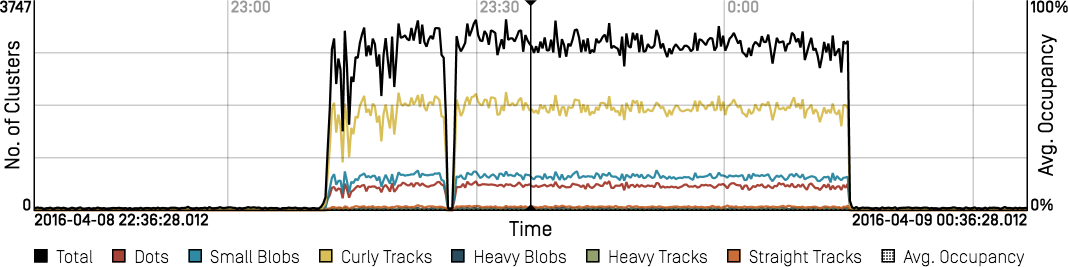
\includegraphics[width=\textwidth]{figures/overview-absolute}
	\caption{Absolute mode.}
	\label{fig:overview-chart-absolute}
	\end{subfigure}

	\vspace{0.2cm}

	\begin{subfigure}{\textwidth}
	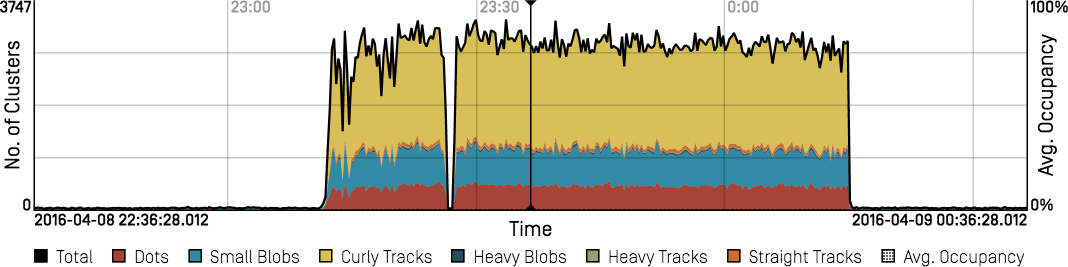
\includegraphics[width=\textwidth]{figures/overview-stacked}
	\caption{Stacked mode.}
	\label{fig:overview-chart-stacked}
	\end{subfigure}

\caption[Comparison of overview rendering modes.]{Example of the same overview chart rendered in different modes.}
\label{fig:overview-chart-modes}
\end{center}
\end{figure}

\begin{description}
	\item[Absolute Mode]
	In this mode (seen in Figure \ref{fig:overview-chart-absolute}), all series of the chart are rendered as points in the plane with respect to the horizontal and vertical axis. Consecutive points of every series are connected by line segments of different color to indicate continuity in time.

	This mode enables users to easily compare values of different series to each other. However, since the experimental data often includes one or two prevailent series, it also frequently overshadows the remaining series as they are rendered over each other, making it harder to read their values.

	\item[Stacked Mode]
	In this mode (seen in Figure \ref{fig:overview-chart-stacked}), the six series corresponding to cluster counts are rendered in a stacked chart, cumulatively adding to each other. Each cluster type series corresponds to a colored area in the chart, while the remaining series are rendered in the same way as in the absolute mode.

	In comparison to the previous mode, this mode distorts the absolute values of the series. It however much better portrays the ratio of representation of one series to another, especially in situations when series have similar values.
\end{description}

\subsection{Main Chart Area}
As the name suggests, the main chart area is the primary section of the UI dedicated to plots of frames from the TPX detectors. By default, it shows only data from a single detector. It can however be configured to partition itself into multiple \textit{cells}, each corresponding to data acquired by a different detector in the network. This feature is often useful on large screens and projectors.

Each cell consists of two square charts, corresponding to individual sensor layers of the detector. Both charts are identical in their layout and internal structure, differing only in the data visualized. Since frames are in their essence pixel matrices, charts visualize them in a standard way by mapping pixel values to different colors, which are later used to fill rectangular areas in the chart. Frame charts can be customized in several ways:

\begin{description}
	\item[Visualized Values]
	If a visualized frame has been captured in the TOT mode, calibration method described in \cite{EnergyCalibration} can be used to obtain energy values from raw counter values. In other operation modes, only counter values are available.

	By default, both charts visualize energy values in the TOT mode and counter values in the other modes. This setting can however be overridden to always visualize counter values in all modes instead.

	\item[Scale Bounds]
	In order to map pixel values to colors, a determinate interval must be specified to establish scale bounds. This interval is by default calculated from the visualized frame automatically. Users can configure its bounds to any fixed values by deactivating the \textit{auto range} checkbox in the details panel.

	\item[Scale Types]
	Given specific scale bounds and values of individual pixels, any function can be used to map absolute values to relative values from a $[0;1]$ interval. By default, a simple linear mapping is used for this task. Users can change this setting to a logarithmic mapping, which better accentuates order differences between individual pixel values in some frames.

	\item[Color Themes]
	The choice of color corresponding to a value between zero and one is purely arbitrary. The visualization UI offers three color themes commonly used in other research programs:

	% CITACE: http://matlab.izmiran.ru/help/techdoc/ref/colormap.html
	\begin{itemize}
		\item The \textit{Jet} theme ranges from blue to red, and passes through the colors cyan, yellow, and orange.
		\item The \textit{Hot} theme varies smoothly from black through shades of red, orange, and yellow, to white.
		\item The \textit{Gray} theme returns a linear grayscale ranging from black to white.
	\end{itemize}
\end{description}

Apart from the listed customizations, frame charts show interactive data labels by responding to mouse movements over the chart area. When the mouse enters the frame, two perpendicular lines are drawn on the pixels underneath the mouse cursor. These lines track the cursor while it hovers over the chart. In addition, several rows of descriptive information are displayed next to the intersection of the lines, giving details on the pixel values and various properties of its associated cluster.

Furthermore, frame charts offer a simple zooming feature. When hovering over the frame area, users can use the drag-and-drop mouse gesture\footnote{The drag-and-drop gesture consists of depressing the left mouse button, dragging the mouse while still holding the button down and then releasing it at a desired position.} to highlight a square portion of the frame. Bounding line segments of this square are then set as the new bounds of the horizontal and vertical axes of the chart. To zoom back, users need to double-click on any position in the frame area.

\subsection{Details Panel}
The details panel is located on the right of the main chart area and consists of multiple auxiliary screens, mostly dedicated to providing further details on the information displayed to the left. The panel is controlled by tabs on the top, each corresponding to a single screen. Only one tab can be selected at any instance. This tab is then highlighted and the respective screen is displayed underneath it.

\begin{description}
	\item[Statistics Screen]
	The statistics screen provides a detailed statistical overview of the currently plotted frames. Should multiple detectors be selected for visualization, it offers an option to select one of the devices as a data source for the overview.

	The statistics consist of two tables. The first table contains cluster counts, calculated on separate rows for every cluster type. Next to the number of clusters, a flux column is displayed. At the bottom of the table, values from both columns are summed together, producing a grand total.

	The second table is displayed only in cases, when the frame has been captured in the TOT mode. It includes a sum of energies from all clusters in the frame and average energy per cluster with a flux column. At the bottom of the table a calculation of instantaneous luminosity from the number of clusters is displayed. This calculation however makes only sense in frames, which are not fully saturated.

	By default, data from both sensor layers are used in the statistical computations. User may however opt to differentiate statistics by individual sensor layers, doubling the amount of figures in both tables.

	\item[Information Screen]
	The information screen displays configuration of the current detector. Similarly to the statistics screen, when multiple detectors are selected, it offers an option to select one of the devices as a data source.

	The displayed information is grouped in several sections. The first section displays time information, such as the start time and the acquisition time of the frame. The following section displays technical information, for example operation mode, frequency of the TPX clock signal and a unique identification of the chip used to capture the frame.

	The last two sections contain secondary information, such as the position and orientation of the detector within the ATLAS machine, or the index information of the ROOT data file, from which the displayed frame has been extracted.

	\item[Filter Screen]
	The filter screen does not show any information. Instead, it allows users to modify displayed data by setting arbitrary predicates. Since most of such predicates operate on numerical measures (for detailed listing, see Section \ref{db:cluster-properties}), they can be specified by defining a minimum and maximum value.

	For convenience, each predicate has an additional switch, which determines if it is active on the current data set. Furthermore, user can activate \textit{the warn mode}, in which a contrasting color is used to highlight all pixels violating the set predicate instead of hiding them.

	When any of the predicates is active, it is not only applied on the displayed charts in the main chart area, but also on the figures displayed on the statistics screen. This is convenient for many applications. To avoid possible confusion, every time predicates are active, a notice is displayed above the statistics screen informing that the values are calculated from only a portion of the frame data.

	In addition to numeric predicates, clusters can be also filtered by shape classification (or by location on pixel matrix). This filtering is achieved by selecting permitted cluster types (or matrix regions) from an exhaustive list of all possible options.

	\item[Settings Screen]
	Similarly to the filter screen, the settings screen does not display any additional information to the user. It merely serves to configure the visualization of the data by enabling or setting various options of the charts.
\end{description}

\subsection{Status Bar}
As in the most UI applications, the status bar is located at the very bottom of the screen. Its primary purpose is to inform users of the current state of the visualization, most notably whether a data download is in progress, or whether the visualization is ready for new commands. In addition, in which every procedure is measured and the time is displayed in the status bar.

\section{Plotting Optimizations}
Since rendering of all charts in the application occurs on the client side, where hardware performance is not guaranteed, the web visualization UI attempts to improve the rendering process as much as possible. This section lists few notable examples of methods used to minimize rendering latency and improve the overall appearance of the plotted output.

\subsection{Prerendering}
Both frame charts and the overview chart offer interactive features. For that reason, their canvases often require to be redrawn upon various user-generated events, such as mouse cursor movements or mouse clicks. Since re-rendering of the entire chart could represent a time-consuming operation, especially on computers with weak hardware, optimization of this procedure is required.

Observant users of the visualization could have noticed that often enough, only a portion the charts in question needs to be redrawn. This can, for instance, be demonstrated on one of the frame charts. When the user's mouse is hovering over the chart, two perpendicular lines forming a cross  appear and track its movements. That would imply that the entire chart is redrawn every time the mouse moves. However, the mouse movement does not affect the data plotted in the chart in any way. To exploit this observation, the chart, which was originally rendered as a whole on a single canvas, is divided into multiple auxiliary canvases, each of them responding to different events.

The auxiliary canvases are transparent, have the same size as the original chart and are laid on top of each other like layers in a photo editor. In addition, every auxiliary canvas maintains an additional bit value signifying whether its state is \textit{valid}. The validity of a canvas can be defined in this context as the state of synchronization between the information drawn on the canvas and the data, which is used to generate such information. Upon different events, some of the auxiliary canvases are invalidated (meaning that their validity bit is set to the \textit{invalid} value). Later on, when the chart is requested to be re-rendered, only those auxiliary canvases, which are invalid, are actually redrawn, saving processor time spent for drawing the remaining canvases.

This technique speeds up the chart rendering significantly, as only portions of charts are redrawn due to UI events. It also implies that every event that affects rendering of UI elements has to come with additional information specifying, which auxiliary canvases need to be invalidated. However, with semantical division of the chart (such as partitioning into data area, scale labels and the mouse cross), this does not seem a complicated task.

\subsection{Pixel Drawing}
One of the UI bugs which proved quite tedious to resolve involved colored rectangles drawn to represent individual pixels of a TPX detector. Given the possibility of zooming, every frame chart has to be able to plot at least $2\times 2$ and at most $256\times 256$ of such pixel rectangles. Since dimensions of the charts adapt to the dimensions of the browser window, every time the window is resized, new dimensions of pixel rectangles need to be calculated.

This calculation is fairly straightforward, but since it utilizes floating-point arithmetic, its results may happen to be imprecise in some cases. And due to this imprecision, pixel rectangles in frame charts used to suffer from periodical fractional offsets, which manifested themselves in the form of a thin grid.

To resolve this issue, the auxiliary canvas responsible for data plots is automatically scaled to size, which is slightly greater than the actual amount of pixels available for rendering, but is a multiple of the number of detector pixels to plot. Consequently, the calculated pixel rectangle dimensions are integer values, and thus allow the usage of \textit{the ImageData API}\footnote{The ImageData API is a part of HTML Canvas API, which allows its users to render pictures by setting values of color components of individual pixels in the bitmap. This approach is faster than the conventional API and guaranteed to not use antialiasing. For more information, see Section 4.12.4.2.16 of \cite{HtmlStandard}.}. After the pixels are rendered in the canvas, it is scaled back down to the exact size of the plot area. At this point, antialiasing is performed. However, since the canvas has already been filled with colored rectangles, there are no transparent pixels from which a grid-like structure could be formed. For that reason, a conventional antialiasing algorithm will produce a satisfying picture.

\subsection{Sub-pixel Rendering}
To render all charts sharply, sub-pixel rendering is supported. Screens with standard pixel resolutions map logical pixels (drawing primitive referenced by the software) to physical pixels (light-emitting devices present in the hardware) bijectively. In comparison, high resolution screens divide their logical pixels uniformly in a way, such that a single logical pixel is displayed by multiple physical pixels. The ratio between the number of physical and logical pixels is defined in the HTML 5 standard \cite{HtmlStandard} as \texttt{devicePixelRatio}\footnote{For instance, Retina display of Apple iPhone 4 has physical resolution $960\times 640$ and logical resolution $480\times 320$. Its pixel ratio is therefore 2.}.

When determining chart sizes prior to rendering, the visualization UI reads the value of the pixel ratio of the current screen and uses it as a coefficient to upscale all canvases accordingly. Contents of charts are then drawn on the canvases, utilizing the enhanced resolution of the screen.

\section{Deployment}
Because the server application consists of two independent daemons, each operating on a different platform, a dedicated deployment method is used. In this section, such method is described in detail.

\subsection{Extension Script Translation}
For coding comfort, the website source makes use of extension languages such as LESS or TypeScript. These languages are respective extensions of the standard CSS and JavaScript, implementing useful features, which are missing or are not supported by their base counterparts. However, since ordinary web browsers are not capable of parsing their advanced syntax, all LESS and TypeScript source files need to be translated by a third-party tool before the web application can be deployed.

The products of the translation process are further optimized for deployment by the process of minification, which removes source code comments, white spaces and obfuscates variable and method names in order to compress file size. Since the code is separated into multiple files, such files are concatenated to minimize the amount of HTTP requests needed to fully load the visualization UI. At the end of this procedure, two compressed files in CSS and JavaScript are generated.

\subsection{Bower Dependencies}
The web application utilizes various open source libraries, most notably jQuery and the Bootstrap Framework. To manage all such dependencies in a well arranged way, the Bower dependency management system is used. The web visualization specifies a \textit{Bower manifest file} in the JSON format. This file lists all dependencies as well as their minimum compatible versions.

When the visualization is deployed, the Bower tool is executed to fetch the latest versions of the required libraries and add their redistributable resources to website contents. This process is deeply integrated with the extension script translation, as the redistributable resources are concatenated with other stylesheets and scripts and minified together. Some dependencies even support strongly-typed bindings in TypeScript. These bindings are downloaded along with the redistributable resources and are used to validate client-side scripts during the translation phase.

\subsection{Grunt Build System}
The Grunt system links all deployment phases together. In a way similar to Makefile, it allows target-driven execution of tasks with possible dependencies and variable arguments. This system is also integrated with the standard Node.js package manager application. To deploy the web visualization UI on the server, two main targets are defined in the application's \textit{Gruntfile}:

\begin{description}
	\item[Production Target]
	The primary purpose of this target is to deploy the web visualization UI with maximum emphasis on speed optimization. All possible files including dependencies are concatenated and minified to minimize loading time of the website in the production environment.

	\item[Debug Target]
	This target is not intended for production use. Its purpose is to maximize readability of the code for the purposes of debugging and development. To achieve this effect, several build phases such as minification and obfuscation are skipped.
\end{description}

\section{Data Import}
Since the JSTP server uses the index database to locate data files based on any given start time, all data files subject to visualization must be stored in the ROOT format and referenced in the \texttt{rootfiles} SQL table.

Accounting for the ever-growing nature of ATLAS-TPX footage, a periodical procedure needs to be performed every time new data arrives from CERN, in order to keep the visualization UI up-to-date. At the time of writing this work, this procedure is semi-automated and initiated manually every day by the researchers at IEAP.

\subsection{Processing Stages}
At CERN, the control PC generates raw data files from the read-out interface of every detector in the network. Data is produced on a hourly basis and saved in the form of multi-frame files. Using FTP, these files are transferred into a temporary directory on the target hard drive. When all file transfers are completed and the validity of files is confirmed, several scripts designed to check consistency of detector acquisition are executed. These scripts analyze contents of received files, reading common configuration values such as the acquisition time or bias voltage, and attempt to find variations between individual frames.

Should these scripts succeed in detecting suspicious values, the files in question are moved into a separate directory and await further inspection by researchers. Otherwise, they move on to the next stage of processing. In this stage, captured frames are subjected to the cluster analysis (for more information about this process, see Section \ref{intro:cluster-analysis}). Should the frames be captured in the TOT mode, at this point calibration data is used in combination with the method described in \cite{EnergyCalibration} to calculate energy values. At the end of this process, ROOT files are produced.

Since the original multi-frame files are not needed anymore, they can be discarded without data loss (or compressed for the purposes of long-term archiving). The ROOT files are moved from the temporary directory to their final location on the hard drive containing the ATLAS-TPX footage database. Subsequently, a dedicated instance of the JSTP data server application is configured to generate information in the index database, in effect registering them for retrieval of JSTP information. From this point onward, the JSTP server as well as the web visualization UI are able to read frames stored within newly added files.

\label{import-automation}
At the present time, the procedure of extending TPX database with new footage is time-consuming as its processing stages often perform similar operations repeatedly for different purposes. For example, a single enumeration of multi-frame files should suffice both for consistency checking and cluster analysis. Furthermore, index data corresponding with produced ROOT files can be generated at the time of their production.

It is however worth noting that this procedure was originally designed in the fall of 2015 with the sole purpose of transferring data from CERN to IEAP. Its automation is currently under investigation.
